\section{API}

\begin{frame}{library design}
	\begin{figure}
		\centering
		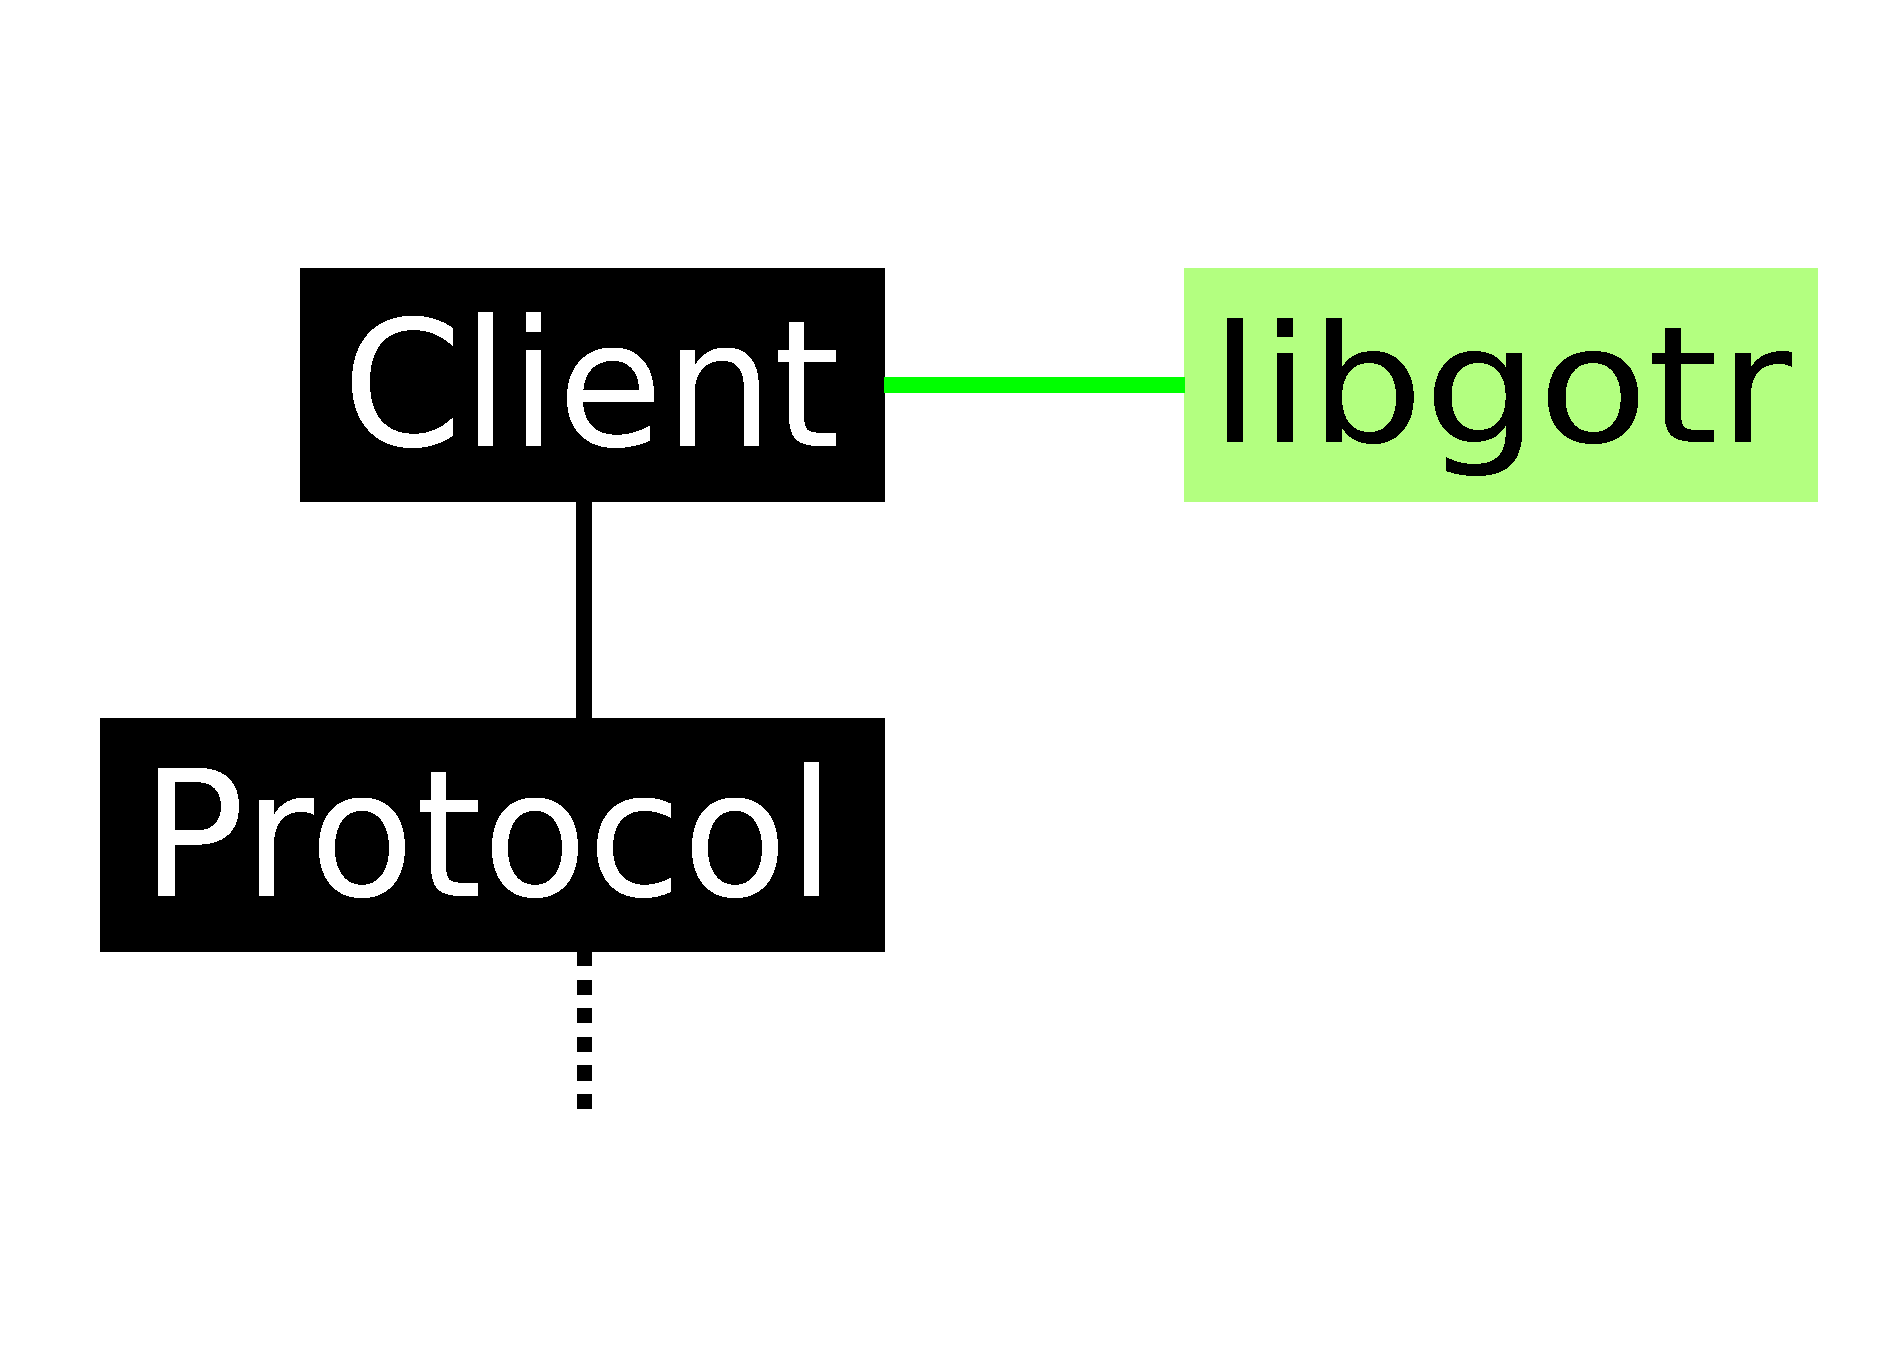
\includegraphics[width = 0.9\textwidth]{./abbildungen/arch_client.eps}
	\end{figure}
\end{frame}

\begin{frame}{library design (alternative)}
	\begin{figure}
		\centering
		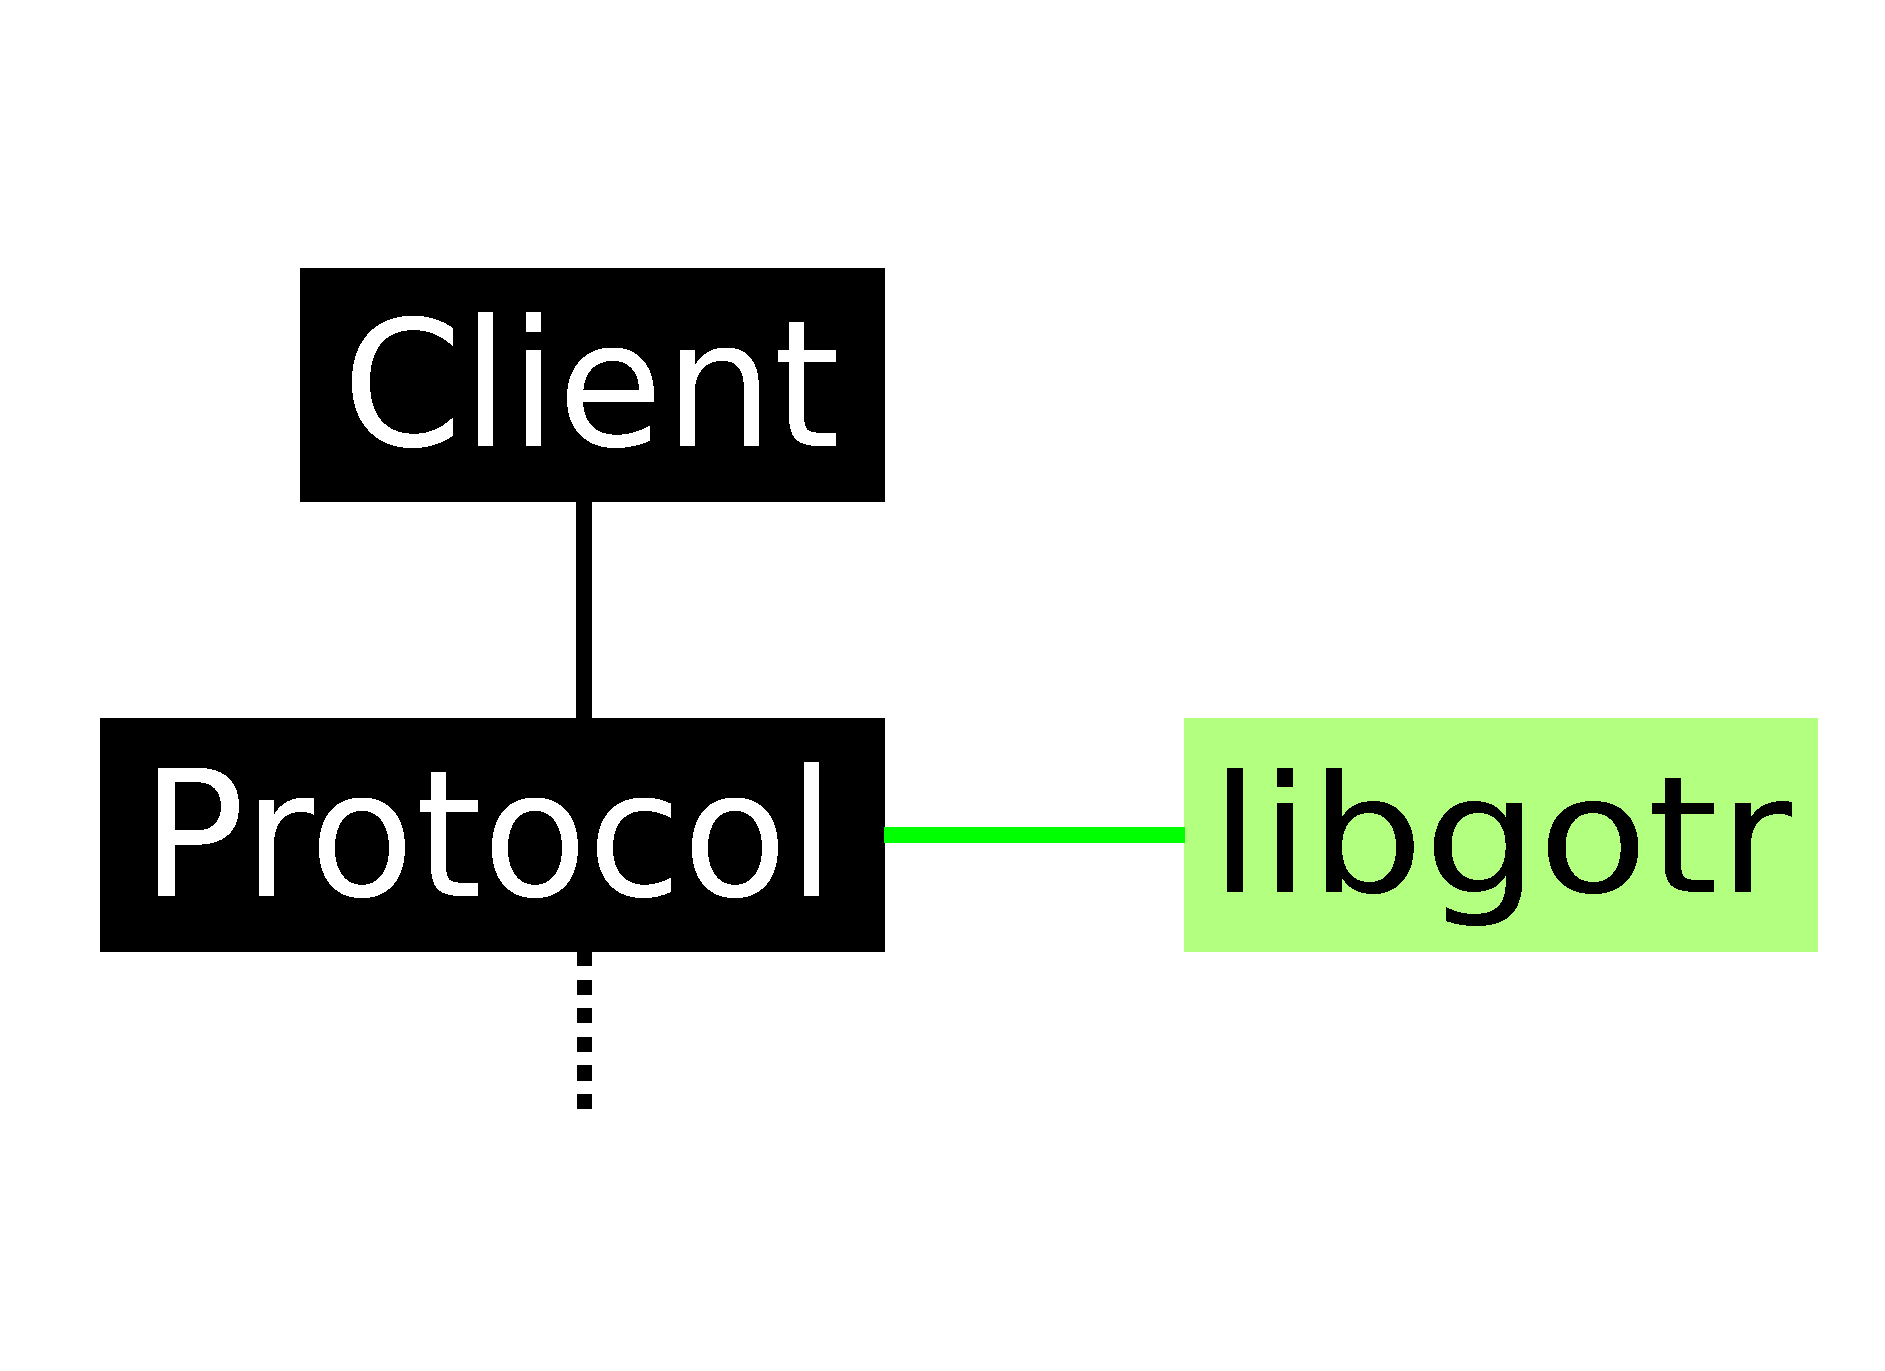
\includegraphics[width = 0.9\textwidth]{./abbildungen/arch_prot.eps}
	\end{figure}
\end{frame}

\lstset{language=C}
\begin{frame}[fragile]{Types}
	\begin{lstlisting}
struct gotr_chatroom;
struct gotr_user;

typedef int (*gotr_cb_send_all)(
    void *room_closure,
    const char *b64_msg);
typedef int (*gotr_cb_send_user)(
    void *room_closure,
    void *user_closure,
    const char *b64_msg);
typedef void (*gotr_cb_receive_user)(
    void *room_closure,
    void *user_closure,
    const char *plain_msg);
	\end{lstlisting}
\end{frame}

\begin{frame}[fragile]{Managing}
	\begin{lstlisting}
struct gotr_chatroom *gotr_join(
    gotr_cb_send_all send_all,
    gotr_cb_send_user send_user,
    gotr_cb_receive_user receive_user,
    const void *room_closure,
    const char *privkey_filename);
struct gotr_user *gotr_user_joined(
    struct gotr_chatroom *room,
    void *user_closure);
void gotr_keyupdate(
    struct gotr_chatroom *room);
void gotr_leave(struct gotr_chatroom *room);
	\end{lstlisting}
\end{frame}

\begin{frame}[fragile]{Messaging}
	\begin{lstlisting}
int gotr_send(
    struct gotr_chatroom *room,
    char *plain_msg);
int gotr_receive(
    struct gotr_chatroom *room,
    char *b64_msg);
struct gotr_user *gotr_receive_user(
    struct gotr_chatroom *room,
    struct gotr_user *user,
    void *user_closure,
    char *b64_msg);
	\end{lstlisting}
\end{frame}
